\chapter{DESENVOLVIMENTO}

\section{Exposição do Tema ou Matéria}

É a parte principal e mais extensa do trabalho detalhando o estudo ou a pesquisa realizada Deve apresentar a fundamentação teórica, a metodologia, os resultados e a discussão. Divide-se em seções e subseções conforme a NBR 6024. Quanto a sua estrutura, segue as recomendações da norma para preparação de trabalhos acadêmicos, a NBR 14724 de 2011. \cite{ABNT} 
Abaixo é apresentada a Figura \ref{fig:estrutura} onde se pode visualizar a estrutura geral do trabalho acadêmico.

\begin{figure}[htb]
	\caption{Estrutura geral}
    \centering
    {\parbox{16cm}{
	    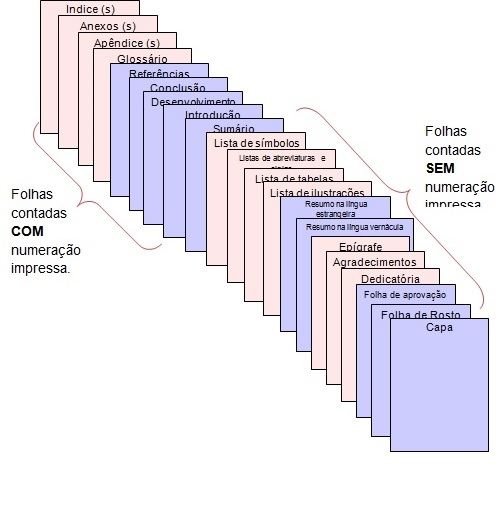
\includegraphics[width=16cm]{images/Fig1.jpg}
        \label{fig:estrutura}
		\fonte{Elaboração das Autoras, 2014}
    }}
\end{figure}


\section{Apresentação Gráfica do Trabalho Acadêmico}

A apresentação gráfica é a definição de tipo de fonte, margens, espaçamento, tipo de papel, etc.

\subsection{Formato (tipo de papel, tamanho da fonte, margens)}

A apresentação gráfica do TC deve seguir os seguintes requisitos:
a) utilizar papel branco ou reciclado, formato A4 (21,0 x 29,7 cm);
b) utilizar o anverso da folha para os elementos pré-textuais;
c) poderá ser utilizado o anverso e verso da folha para impressão dos elementos 
    textuais e pós-textuais;
c) digitar o texto na cor preta;
d) fonte tamanho 12 para o texto;
e) fonte tamanho 10 para citações longas, notas de rodapé, legendas e fontes 
    (identificação) das ilustrações e tabelas e paginação;
f) optar por fontes arredondadas (Times New Roman ou Arial);
g) adotar as margens:
    - para o anverso da folha:
       - superior de 3 cm, 
       - inferior de 2 cm,
       - esquerda de 3 cm,
       - direita de 2 cm,
     - para o verso:
        - superior de 3 cm, 
        - inferior de 2 cm,
        - esquerda de 2 cm,
       - direita de 3 cm,
h) primeira linha do parágrafo com recuo de 2 cm a partir da margem esquerda;
          i) citação longa (com mais de três linhas) com recuo de 4 cm a partir da margem
    esquerda;
j) nota de rodapé digitada dentro das margens indicadas, devendo ficar separada do 
   texto por um traço de 5 cm a partir da margem esquerda.

\subsection{Espaçamento}

O espaçamento que você deve adotar na formatação é:
a) espaço 1,5  - todo o texto,
          b) um espaço de 1,5;
     - separa o texto da citação longa,
     - separa cada título das seções e subseções do texto que os precedem e que os 
       sucedem,
c) espaço simples para;
    - citações longas,
    - notas de rodapé,
    - referências,
    - legenda e fonte das ilustrações e tabelas,
    - natureza do trabalho.
e) um espaço simples -  entre uma referência e outra, na lista de referências ao final do trabalho.

\subsection{Indicativo de seção e numeração progressiva}

Seção é a divisão do TC, aplicada somente aos elementos textuais e visa expor numa sequência lógica o relacionamento da matéria e a permitir a sua localização. De acordo com a NBR 6024 as seções também podem ser subdividas em subseções.
A seção primária é a principal divisão do texto do TC, que sempre deverá ser grafada em números inteiros a partir do 1, alinhados à esquerda por um espaço de caractere e iniciar em página distinta e ímpar (anverso). As demais são chamadas de subseções e/ou seções secundária, terciária, quaternária e quinária. Se for necessário enumerar os diversos assuntos de uma seção que não possua título, esta deve ser subdividida em alíneas. As alíneas são ordenadas alfabeticamente e terminam em ponto e vírgula, exceto a última que termina em ponto. Todas as seções devem conter um texto relacionado a elas (FIGURA \ref{fig:secoes}) .
Exemplo sugerido pelo IFC:
1 SEÇÃO PRIMÁRIA (maiúsculas em negrito)
1.1 SEÇÃO SECUNDÁRIA (maiúsculas)
1.1.1 Seção terciária (em negrito com primeira letra maiúscula)
1.1.1.1 Seção quaternária (primeira letra maiúscula)
1.1.1.1.1 Seção quinária (em itálico com primeira letra maiúscula)
a) alínea (primeira letra minúscula);
b) alínea;
    - subalínea.
c) alínea.
2 SEÇÃO PRIMÁRIA 
2.1 SEÇÃO SECUNDÁRIA 
2.1.1 Seção terciária 
.
.
.
\begin{figure}[htb]
	\caption{Seções}
    \centering
    {\parbox{16cm}{
		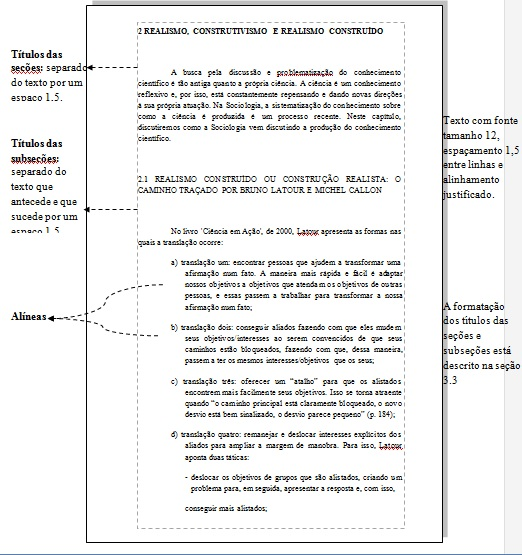
\includegraphics[scale=1.1]{images/Fig2.jpg}
	    \label{fig:secoes}
	    \hspace{0.0cm}{Fonte: Elaboração das Autoras, 2014}
    }}
\end{figure}


\subsection{Paginação}

Para o TC, as páginas pré-textuais devem ser contadas, mas não numeradas. A contagem será a partir da folha de rosto. A numeração deve configurar a partir da primeira folha textual em algarismos arábicos e sendo sequencial até o final do trabalho. 
A paginação da(s) referência(s), do(s) anexo(s) e do(s) apêndice(s) deve ser numerada sequencialmente no TC. As páginas que não permitem a inclusão de números também são contadas (mapas, documentos, ilustrações, etc.).
O número da página deve aparecer no canto superior direito da folha, a 2 cm da borda superior, ficando o último algarismo a 2 cm da borda direita da folha.
Para trabalhos com mais de um volume, a numeração sequencial das folhas deve ser mantida. Se o trabalho contiver apêndice e anexo, a numeração das páginas deve dar sequência ao texto principal.

\subsection{Lombada}

A lombada é um elemento opcional para o TC e na sua estrutura, deve conter os seguintes elementos: 
a)	nome(s) do(s) autores, quando houver;
b)	título;
c)	identificação do volume, fascículo e data, se houver.
Todos os elementos que compõem a lombada devem ser centralizados em suas áreas, com fonte tamanho 12, espaçamento simples e todas as letras maiúsculas (FIGURA \ref{fig:lombada}).

\begin{figure}[h]
	\caption{Lombada}
    \centering
    {\parbox{16cm}{
		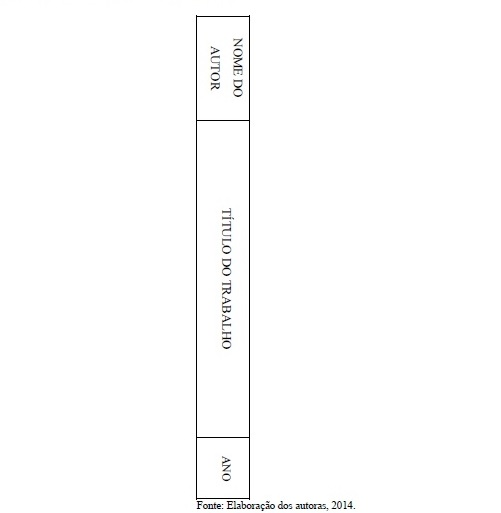
\includegraphics[scale=1.1]{images/Fig3.jpg}
	    \label{fig:lombada}
	    \hspace{5.7cm}{Fonte: Elaboração das Autoras, 2014}
    }}
\end{figure}

% 
%--------- FIM DESENVOLVIMENTO------------
%